\documentclass[13pt]{article}
\renewcommand{\baselinestretch}{1.0}
\usepackage[utf8]{vietnam}
\usepackage[a4paper, total={6in, 8in}]{geometry}
\usepackage[vietnamese,english]{babel}
\usepackage{hyperref}
\usepackage{mathtools}
\usepackage{amssymb}
\usepackage{indentfirst}
\usepackage{graphicx}
\usepackage{minted}
\usepackage{ragged2e}
\usepackage[nottoc]{tocbibind}

\hypersetup{
    colorlinks=true,
    linkcolor=blue,
    citecolor=blue,
    urlcolor=blue,
}
\begin{document}
\begin{titlepage}
    \begin{center}
        \vspace*{1.8cm}
        \Large
        Distributed System Labwork 2\\
        \Large
        \vspace{0.5cm}
        \begin{center}
            
\includegraphics[scale=1.0]{logo USTH-01.PNG}
        \end{center}  
        \vspace{0.5cm}
            Group 6 - ICT\\
        \vspace{0.5cm}
            University of Science and Technology of Hanoi\\
        \vspace{0.5cm}
            January, 2022
        \vfill
          
   \end{center}
\end{titlepage}

\newpage
\tableofcontents
\newpage

\section{Introduction}
\subsection{Overview}
\noindent%
We try to develop a file transfer using RPC in this lab. In this lab, we'll utilize the letter C.

\subsection{Protocol}

\begin{figure}[h]
    \centering
    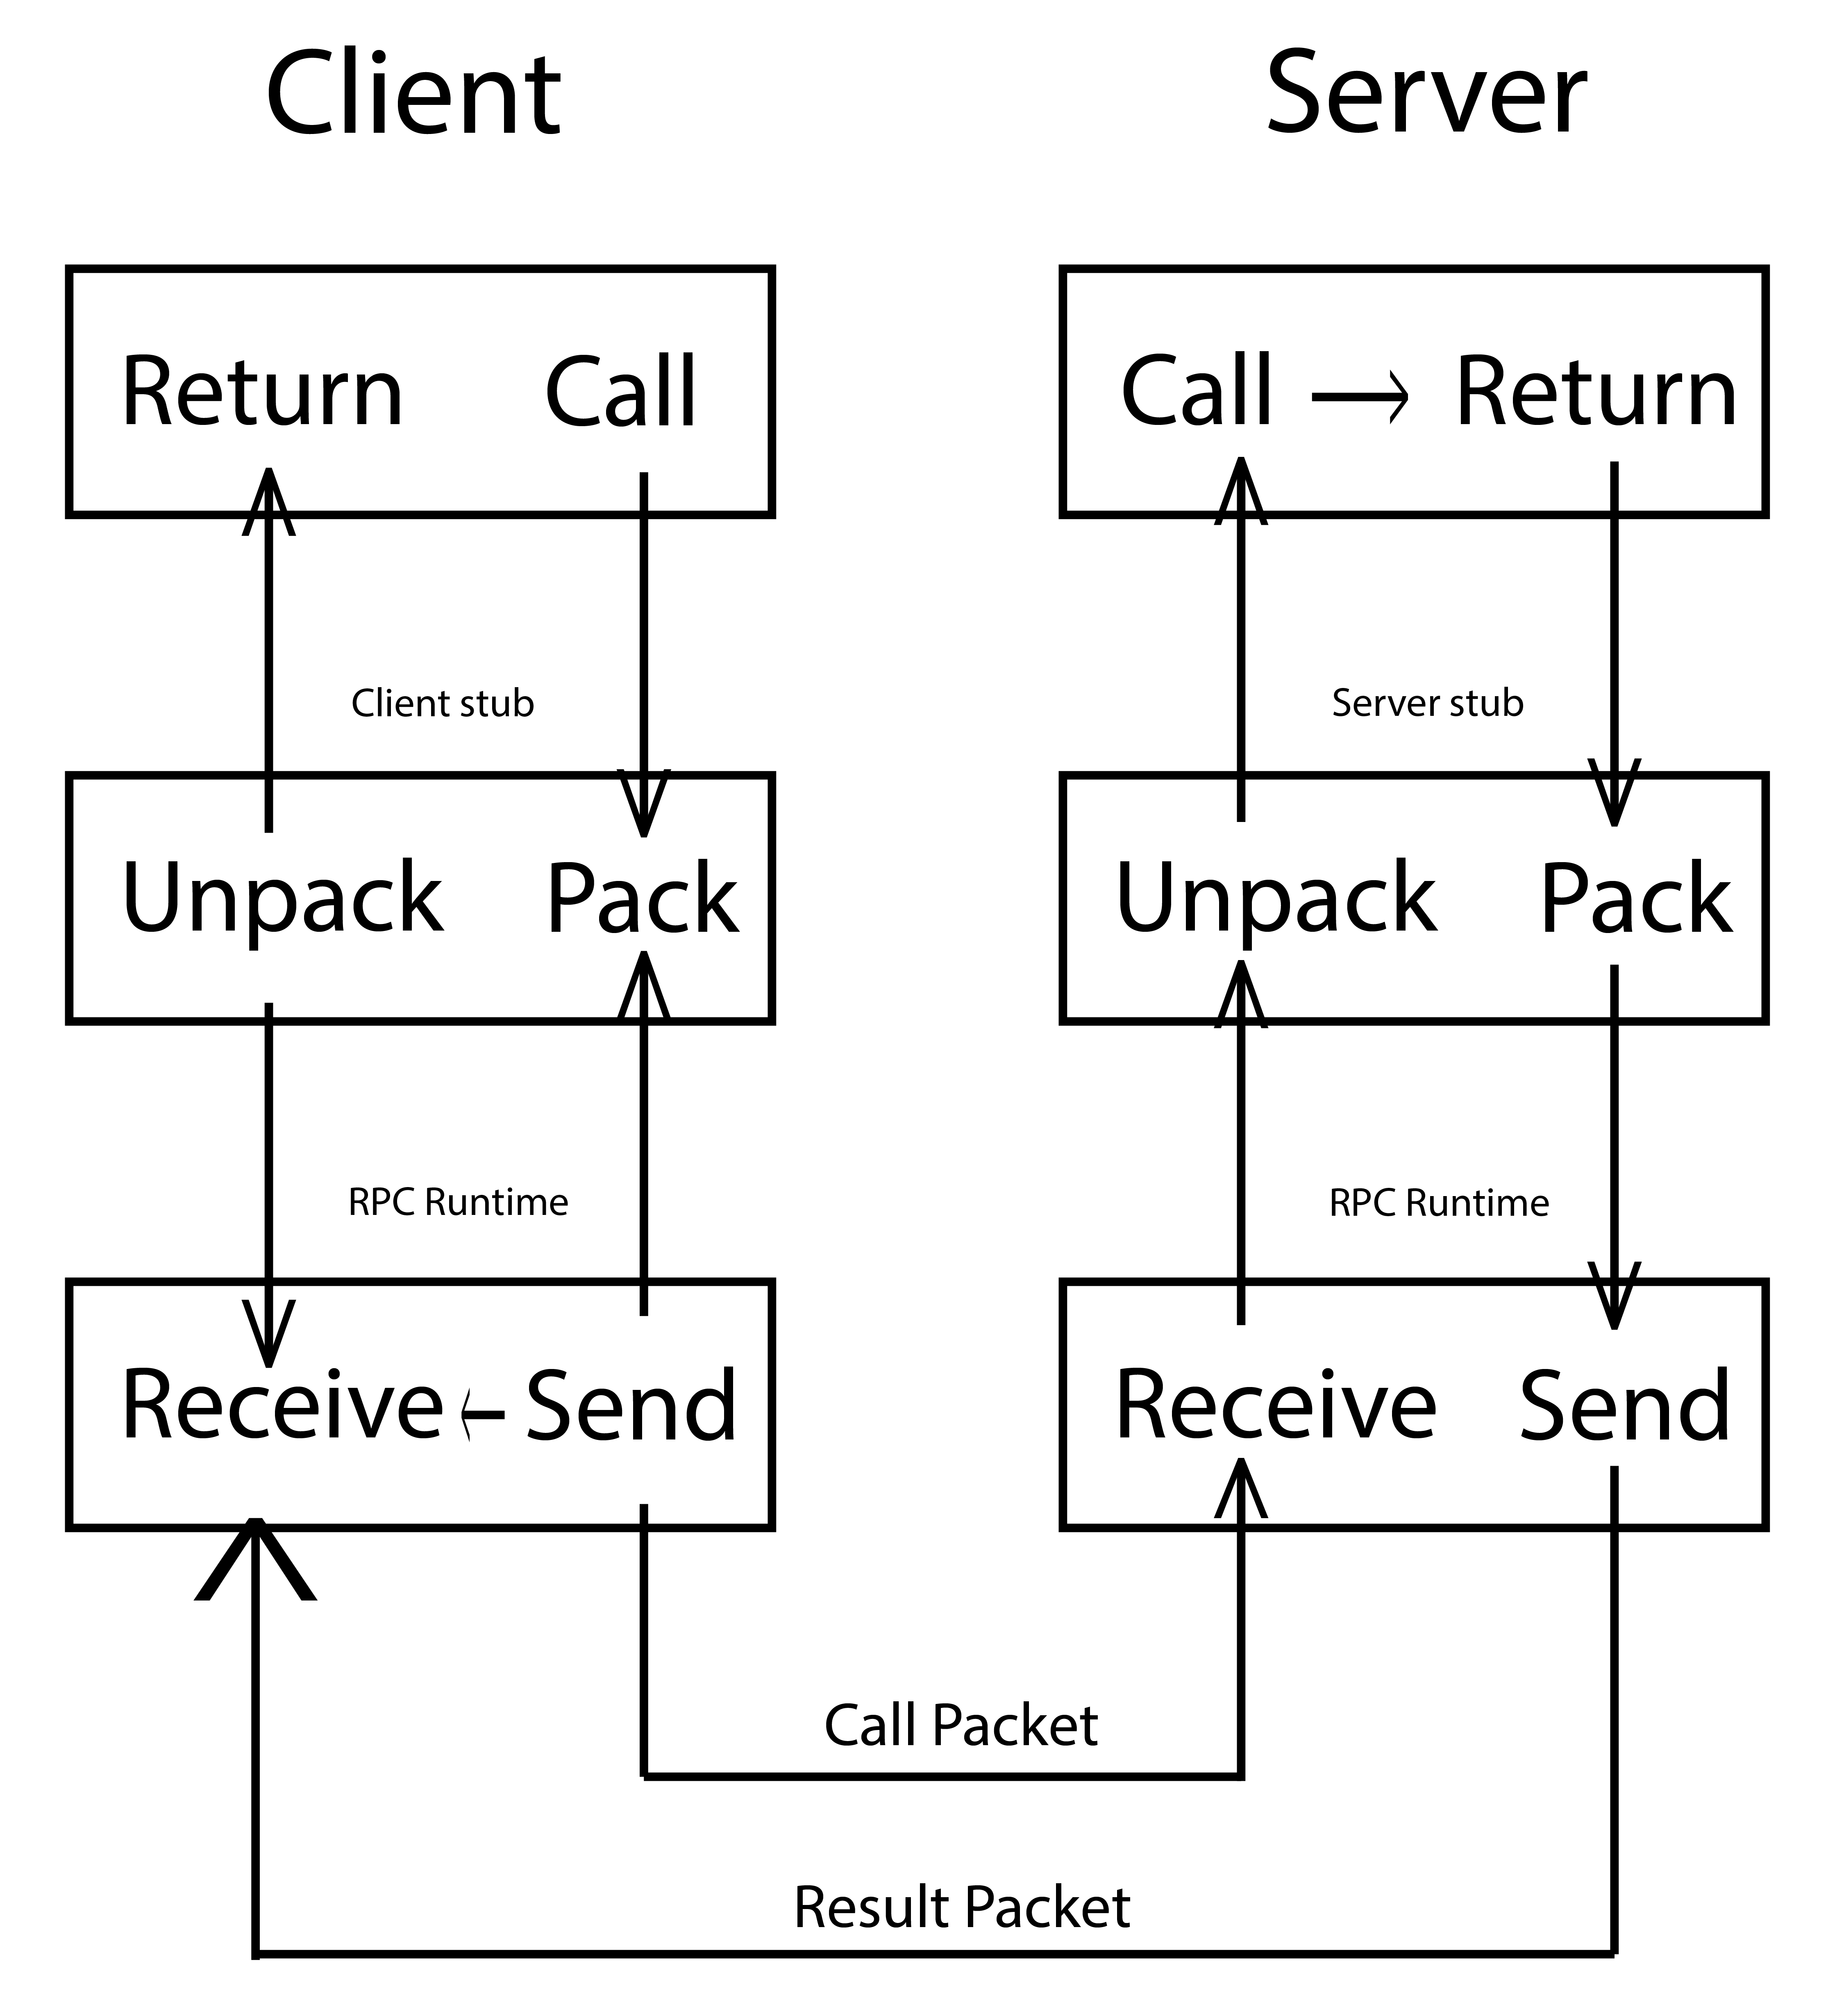
\includegraphics[scale=0.2]{protocol_diagram-01.png}
    \caption{Protocol diagram}
    \label{fig:protocol}
\end{figure}

\begin{itemize}
    \item The client sends a message to the client stub. The client stub packs the parameters into a message and performs a system call to deliver the message. The client's local operating system transfers the message from the client machine to the server machine.
    \item The server's local operating system forwards incoming packets to the server stub.
    \item The server stub unpacks the message's arguments.
    \item Finally, the server operation is invoked by the server stub.
\end{itemize}

\subsection{System organization}
\noindent%
The client and the server connects through UDP.

\begin{figure}[H]
    \centering
    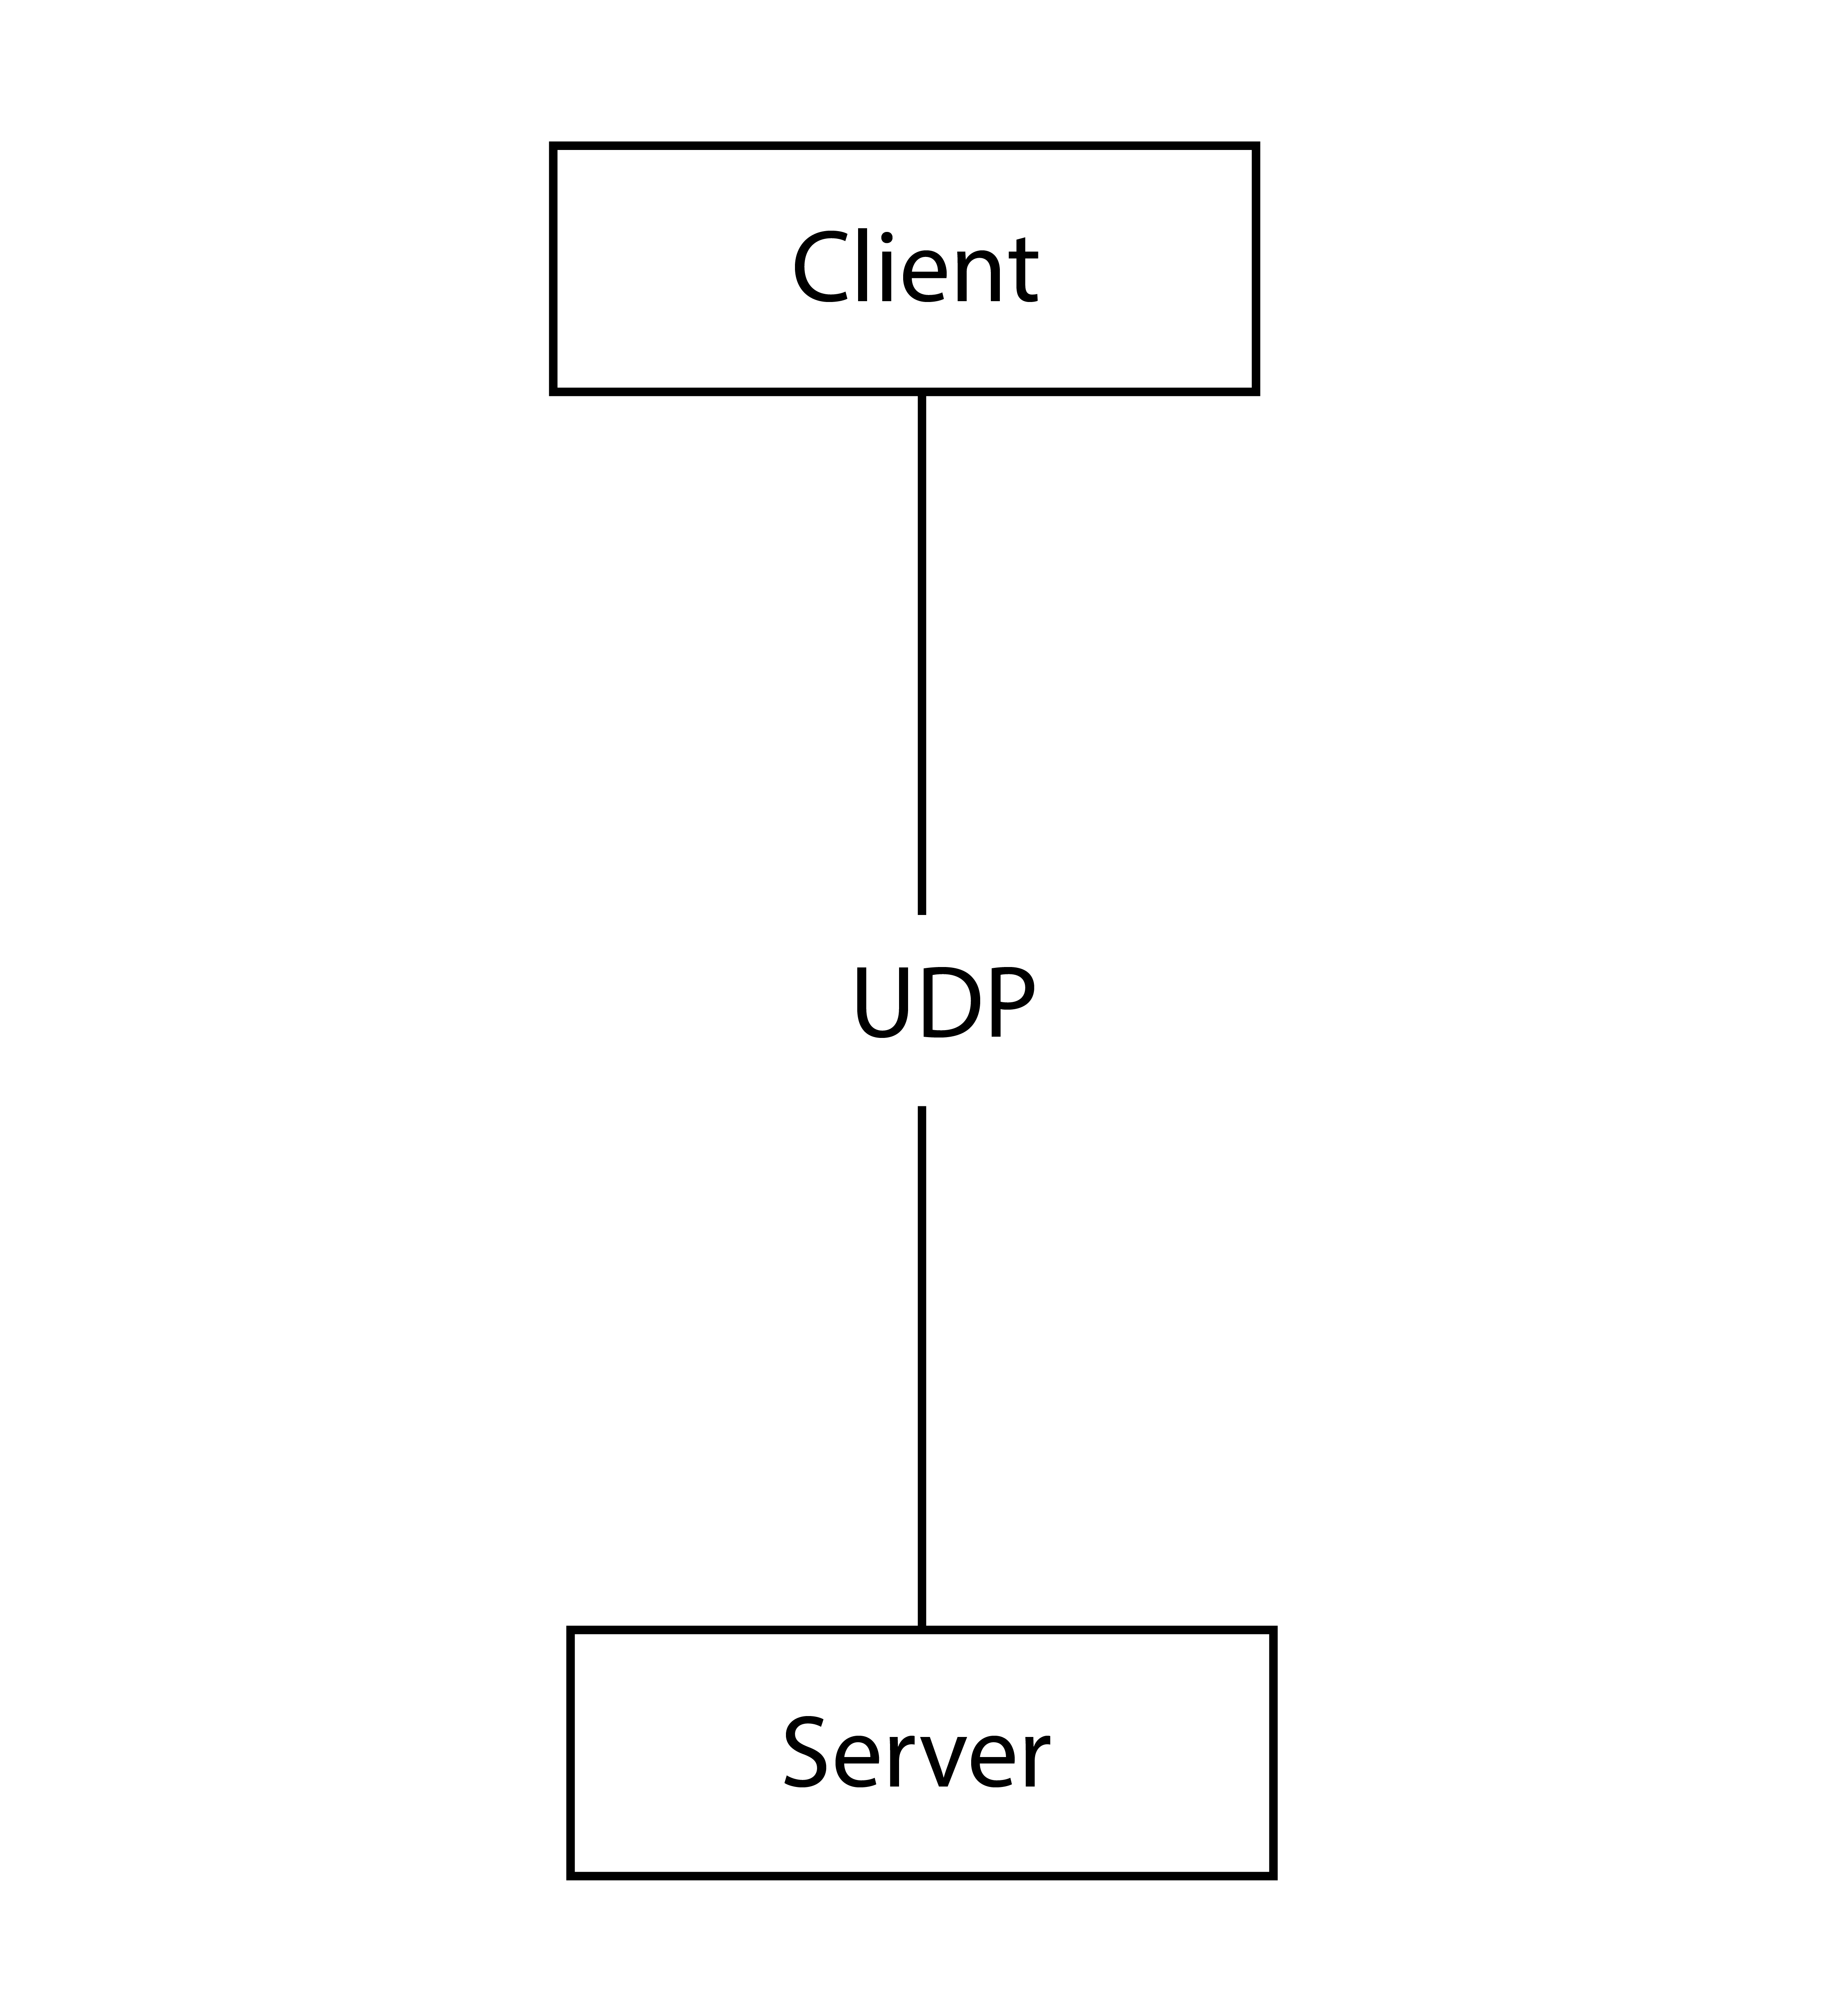
\includegraphics[scale=0.25]{system-01.png}
    \caption{System organization}
\end{figure}

\subsection{Implementation}
\noindent%
At first, we created a file a named it file.x. The code in the file was implemented below:

\begin{minted}{c}
struct file {
	char filename[1024];
	char buffer[1024];
	int buffer_size;
};

program FILE_TRANSFER_PROG {
	version FILE_TRANSFER_VERS {
		int transfer_file(file) = 1;
	} = 1;
} = 0x20000001;
\end{minted}

\noindent%
Client and server stubs were generated when we typed "rpcgen -a -C file.x". \\

\noindent%
We have implemented the client side:
\begin{minted}{c}
#include <unistd.h>
#include <stdio.h>
#include <stdlib.h>
#include <string.h>
#include <sys/types.h>
#include <sys/socket.h>
#include <netdb.h>

int main(int argc, char* argv[]) {
    int so;
    char s[100];
    struct sockaddr_in ad;

    socklen_t ad_length = sizeof(ad);
    struct hostent *hep;

    // create socket
    int serv = socket(AF_INET, SOCK_STREAM, 0);

    // init address
    hep = gethostbyname(argv[1]);
    memset(&ad, 0, sizeof(ad));
    ad.sin_family = AF_INET;
    ad.sin_addr = *(struct in_addr*)hep->h_addr_list[0];
    ad.sin_port = htons(12345);

    // connect to server
    connect(serv, (struct sockaddr*)&ad, ad_length);
    
    memset(&s, 0, 100);
    FILE* file;
    file = fopen("send_file.txt", "r");
    if (file == NULL) {
    	printf("The file is null");
    } else {
    	printf("Read file successfully\n");
    }
    
    char buffer[1024] = {0};
    while (fgets(buffer, sizeof(buffer), file) != NULL) {
    	int i = send(serv, buffer, sizeof(buffer), 0);
    	if (i == -1) {
    		printf("Send data fail");
    	}
    	memset(&buffer, 0, sizeof(buffer));
    }
    printf("File sent!");
    
    close(serv);
    return 0;
}
\end{minted}

\noindent%
We have implemented the server side:

\begin{minted}{c}
#include <stdio.h>
#include <stdlib.h>
#include <string.h>
#include <sys/types.h>
#include <sys/socket.h>
#include <netdb.h>
#include <unistd.h>

int main() {
    int ss, cli, pid;
    struct sockaddr_in ad;
    char s[100];
    socklen_t ad_length = sizeof(ad);

    // create the socket
    ss = socket(AF_INET, SOCK_STREAM, 0);

    // bind the socket to port 12345
    memset(&ad, 0, sizeof(ad));
    ad.sin_family = AF_INET;
    ad.sin_addr.s_addr = INADDR_ANY;
    ad.sin_port = htons(12345);
    bind(ss, (struct sockaddr*)&ad, ad_length);

    // then listen
    listen(ss, 0);

    while (1) {
        // an incoming connection
        cli = accept(ss, (struct sockaddr*)&ad, &ad_length);

        pid = fork();
        if (pid == 0) {
            // I'm the son, I'll serve this client
            printf("client connected\n");
            
            FILE* file;
            file = fopen("recieve_file.txt", "w");
            if (file == NULL) {
            	printf("Cannot open file");
            } else {
            	printf("Start writing file\n");
            }
            
            char buffer[1024];
            while (1) {
                int i = recv(cli, buffer, sizeof(buffer), 0);
                if (i <= 0) {
                	break;
                }
                fprintf(file, "%s", buffer);
                memset(&buffer, 0, sizeof(buffer));
            }
            printf("File received!");
            
            return 0;
        } else {
            // I'm the father, continue the loop to accept more clients
            continue;
        }
    }
    // disconnect
    close(cli);
    close(ss);

}
\end{minted}

\subsection{Contribution}
\noindent%
\begin{table}[ht!]
  \begin{center}
    \label{tab:table1}
    \begin{tabular}{l|l}
      \textbf{Member} & \textbf{Contribution}\\
      \hline
      Nguyen Quang Vinh & Client code\\
      Nguyen Tran Nguyen & Server code\\
      Mai Xuan Hieu & Design Protocol\\
      Nguyen Anh Quan & Design Architecture\\
      Nguyen Tuong Quynh & Report\\
    \end{tabular}
    \caption{Contribution Table}
  \end{center}
\end{table}
\end{document}